\section{Understanding Pointers, Memory Management, Stacks, and Arrays in C}

\subsection{Pointers}
Pointers are a type of variable that contain memory addresses. A pointer in C is declared by prefixing the variable name with an asterisk (\texttt{*}). For example:
\begin{lstlisting}
int *i; // pointer to an integer
char *c; // pointer to a character
\end{lstlisting}

There are two main operations that can be performed with a pointer:
\begin{itemize}
    \item Change the content at the memory address the pointer points to.
    \item Change the address that the pointer points to.
\end{itemize}

\noindent Consider the following example:
\begin{lstlisting}
int var = 123;
int *i;
i = &var; // pointer i points to the address of var
*i = 5;  // the content at the address pointed by i is changed to 5
\end{lstlisting}

After execution, \texttt{var} will be 5.

\begin{figure}[h!]
    \centering
    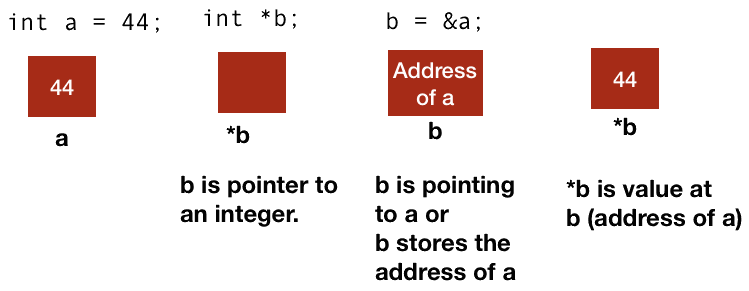
\includegraphics[width=0.8\textwidth]{images/pointers_c.png}
    \caption{Pointers in C.}
\end{figure}

\subsection{Memory Management in C}
During the execution of a program, memory in C is managed in two ways:
\begin{itemize}
    \item \textbf{Static Memory Management}: A fixed memory area is allocated by the operating system for the entire duration of the program.
    \item \textbf{Dynamic Memory Management}: Two distinct memory areas are allocated and used as needed: the stack and the heap.
\end{itemize}

\subsubsection{Stack}
The stack in C is a special region of a program's memory that stores temporary variables created by each function (including the \texttt{main} function). It plays a crucial role in managing function calls, local variables, and control flow.
The stack is used for variables and function parameters. For each function call, a new stack frame is created with its parameters. When the function completes, its stack frame is removed, and the stack reverts to its previous state. The stack operates on the Last In, First Out (LIFO) principle. This means that the last item pushed onto the stack is the first one to be popped off. Think of it like a stack of plates: you can only add or remove the top plate.

\begin{figure}[h!]
    \centering
    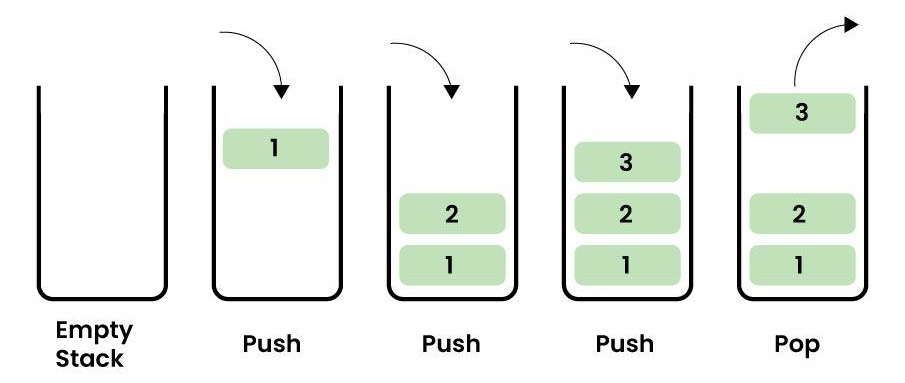
\includegraphics[width=0.8\textwidth]{images/lifo.jpg}
\end{figure}

\paragraph{Heap}
The heap is a memory area managed by the programmer and can be dynamically allocated as needed using C's memory management libraries.

\begin{itemize}
    \item The \textbf{ESP} (Extended Stack Pointer) register points to the top of the current stack frame. It keeps track of the last used location in the stack. When a function is called, the ESP is adjusted to allocate space for the function's local variables. When a function returns, the ESP is adjusted back to free the space.
    \item The \textbf{EBP} (Extended Base Pointer) register points to the base of the current stack frame. EBP is used to reference function parameters and local variables in a consistent way, even if the ESP changes during the function execution (e.g., due to push and pop operations). When a function is called, the current EBP value is pushed onto the stack, and EBP is then set to the current value of ESP.
    \item The \textbf{EIP} (Extended Instruction Pointer) register holds the address of the next instruction to be executed. When a function call occurs, the current EIP (pointing to the next instruction in the calling function) is pushed onto the stack. This allows the program to return to the correct place after the function call completes. This push operation saves the address of the next instruction to be executed after the function returns, facilitating the call-return mechanism.
\end{itemize}

\paragraph{Stack Operation during a Function Call}
\begin{enumerate}
    \item Function Call (CALL Instruction): When a function is called, the current EIP (instruction pointer) is pushed onto the stack. This saves the address of the instruction to return to after the function completes. The current EBP is also pushed onto the stack to preserve its value. ESP is decremented to make space for the local variables and the function's stack frame.
    \item Function Prologue: The new function sets its EBP to the current ESP value to establish a new base for its stack frame. Local variables and saved registers are pushed onto the stack as needed.
    \item Accessing Parameters and Local Variables: Function parameters are accessed at positive offsets from EBP. Local variables are accessed at negative offsets from EBP.
    \item Function Return (RET Instruction): The ESP is restored to the value of EBP to free the stack frame. The previous EBP is popped off the stack to restore the caller's base pointer. The saved EIP (return address) is popped from the stack into the EIP register to resume execution at the point after the function call.
\end{enumerate}

\paragraph{Example of Stack Usage}

Consider the following C code:

\begin{lstlisting}
void func(int a, int b) {
    int x, y;
    x = a + b;
    y = x * 2;
}

int main() {
    int p = 5, q = 10;
    func(p, q);
    return 0;
}
\end{lstlisting}

Here’s how the stack operations would work:

\begin{itemize}
    \item \textbf{Calling \texttt{func(p, q)}}:
    \begin{itemize}
        \item The current EIP (address of the next instruction after the call) is pushed onto the stack.
        \item The current EBP is pushed onto the stack.
        \item ESP is adjusted to allocate space for \texttt{func}'s stack frame.
    \end{itemize}
    \item \textbf{Inside \texttt{func}}:
    \begin{itemize}
        \item EBP is set to the current value of ESP.
        \item Space is allocated for local variables \texttt{x} and \texttt{y} on the stack by adjusting ESP.
        \item Parameters \texttt{a} and \texttt{b} are accessed relative to the new EBP.
    \end{itemize}
    \item \textbf{Returning from \texttt{func}}:
    \begin{itemize}
        \item ESP is restored to the value of EBP.
        \item The previous EBP is popped from the stack.
        \item The saved return address (EIP) is popped from the stack, and execution resumes in \texttt{main}.
    \end{itemize}
\end{itemize}


\paragraph{Visualization}

Here’s a simplified visualization of the stack state at different stages:

\begin{enumerate}
    \item Initial State (Before Function Call)

\begin{verbatim}
| High Address | ...       |
|              |           |
|              |           |
| Low Address  | ...       |
\end{verbatim}

\item After Pushing Return Address and EBP

\begin{verbatim}
| High Address | ...       |
|              | Return EIP|
|              | Old EBP   |
| Low Address  | ...       |
\end{verbatim}

\item Inside Function (After Allocating Local Variables)

\begin{verbatim}
| High Address | ...       |
|              | Return EIP|
|              | Old EBP   |
|              | Local var |
|              | Local var |
| Low Address  | ...       |
\end{verbatim}
\end{enumerate}


The stack in C is a critical component of memory management, enabling function calls, local variable storage, and control flow management. Understanding the stack's LIFO nature, the role of registers like ESP, EBP, and EIP, and the operations performed during function calls and returns is essential for effective programming and debugging in C.

\subsection{Arrays in C}
C provides arrays, which are sequences of homogeneous elements. An array in C is declared as follows:
\begin{lstlisting}
int array[10]; // array of 10 integers
\end{lstlisting}

Each element in the array is accessible via its index, starting from 0. For example:
\begin{lstlisting}
array[0] = 1;
array[9] = 10;
\end{lstlisting}

\subsection{Multidimensional Arrays}
C also supports multidimensional arrays, such as matrices. A multidimensional array is defined as:
\begin{lstlisting}
int matrix[3][3]; // 3x3 matrix
\end{lstlisting}

Each element is accessed using two indices (row and column). For example:
\begin{lstlisting}
matrix[0][0] = 1;
matrix[2][2] = 9;
\end{lstlisting}

The concepts for manipulating multidimensional arrays are similar to those for one-dimensional arrays, with the addition of multiple indices.
